\documentclass[]{article}

\usepackage{graphicx}
\usepackage{color}


\setlength{\parindent}{0em}
\setlength{\parskip}{1em}


\begin{document}

%\maketitle


\section*{Response to Reviewer 1}

We thank the reviewer for his/her constructive comments and are pleased with the positive assessment or our work. We have addressed the specific comments made by the reviewer as described below. We hope that the revised manuscript can now be accepted for publication.

\dotfill

\textbf{1. Reviewer:} \textit{One comparison that came to mind reading the paper, is that the results show very little value in optimizing the most-downstream turbines, and in general, improvement in power comes from modifications upstream, and that self-optimization is not possible. This stands in contrast to a result such as:}
	
\textit{Ciri, Umberto, Mario Rotea, Christian Santoni, and Stefano Leonardi. “Large Eddy Simulation for an Array of Turbines with Extremum Seeking Control.” In American Control Conference. Boston, MA, 2016. }
	
\textit{Where the TSR of downstream turbines is re-optimized for wake conditions (and the upstream turbine is left as is at the end of the optimization). It would seem the difference in modeling methods and/or how turbine control is implemented yields the different results, but I believe it would be worth discussing the difference, for example around the paragraph beginning with "The figure shows that the first row (R1)..." on page 12.}

\textbf{Response:} This is an interesting comment. It is correct that this contrast results from the way turbines and their controls are modeled in the current study and that of Ciri et al. The reference disk-based thrust coefficient $C_T' = 2$ used here actually implies intrinsic self-optimization of blade pitch and generator torque to local flow conditions, even though these actions are not resolved by our current actuator disk formulation which directly controls $C_T'$. In case these degrees of freedom would be resolved, for instance using an actuator line model as in Ciri et al., the ESC from the latter study could e.g. be used to optimize torque controller gain in order to achieve an effective $C_T' \approx 2$. 

We have included the fact that the reference case already implies self-optimization in the revised manuscript as follows (p 4, l. 21): 

``
A conventionally (greedily) controlled wind farm with steady $C_T' = 2$ was defined as a reference case. \textbf{Note that this would correspond to a farm with ideal turbines for which generator torque is being controlled dynamically to track the maximum power point at the Betz limit perfectly.} Several different optimal control cases were defined, ...
''

However, even given the discussion above, it is not unimaginable that a turbine could temporarily outperform this greedy control setting, e.g. by timely reacting to incoming flow accelerations. This is what we would refer to as self-optimization. {\color{blue} We have explicitly defined this in the text as follows (p ??):

``
...This suggests that self-optimization \textbf{(i.e. temporarily outperforming conventional greedy control in response to incoming flow events)} is very limited: the optimal controls for a given turbine are designed to create ...
'' }

(IS DIT OKE?? Kan het deel in blauw misschien beter gewoon weglaten?)


\dotfill

\textbf{2. Reviewer:} \textit{Figure 3/related text: Would another way to describe Ct2 vs Ct3 be that Ct2 can only lower the thrust, while Ct3 is allowed to raise it?}

\textbf{Response:} Indeed, this is correct. We have mentioned this explicitly in the revised manuscript as follows (p. ??, l. ??):

``
... and the maximal thrust coefficient $C_{T,\rm max}' = 2$ or 3, \textbf{with thrust forces that can respectively only be reduced (underinductive), or also increased (overinductive) compared to the Betz optimum at $C_T' = 2$} (see Eq. 5). 
''

\dotfill

\textbf{3. Reviewer:} \textit{``... NREL 5MW rotor with a 50\% increase in chord length ...'' does this imply the method is currently assuming the chord length is variable? Could this not be achieved by a change in pitch angle?}

\textbf{Response:} No, the method does not imply a variable chord length. 

Current turbines are designed to approach maximum $C_T'$ values around 2, corresponding to the Betz limit. Aiming to increase thrust by adapting the pitch angle would inevitably lead to severe efficiency losses due to stall on the turbine blades. Therefore, we provide an example of how an alternative turbine design (i.e. with an increased chord length and operational TSR) could attain a maximum $C_T'$ of 3.5. Given such a turbine design, achieving thrust ratings $C_T' < 3.5$ is straightforward by pitching blades towards the feather position. 

We have slightly modified the statement in the revised manuscript to avoid any confusion with regard to possibly having the chord length as a control variable. (p. ??, l. ??):

``
The resulting maximum thrust coefficient of 3.5 can, e.g., be \textbf{attained by the NREL 5MW turbine with a slight modification in the rotor design}, i.e. a 50\% increase in blade chord length and an operational tip speed ratio 25\% higher than 
the original design value (see Goit and Meyers, 2015, Appendix A). \textbf{Furthermore, given such redesign, dynamic reductions from this value could be realized through blade pitch control, for which actuation in the order of $10^\circ/$s is possible (see, e.g., Jonkman et al. 2009).} 
''

Note that this control strategy is not unique and is solely given as an indication for the technical feasibility of tracking the proposed $C_T'$ waveform. In practice, we expect that this can also be achieved through a combination of generator torque and blade pitch control. This is subject of ongoing investigation.


\clearpage
\section*{Response to Reviewer 2}
We thank reviewer 2 for reading our work and for providing detailed feedback which has improved the quality of the manuscript. We are pleased with his/her positive assessment of our research and have addressed the specific comments in the manuscript as described below. We hope that the revised manuscript can now be accepted for publication. 

\dotfill

\textbf{Reviewer: } \textit{...LES setup is described/illustrated properly - except of the characteristics of the turbines/actuator disks considered. Would be nice to have the size of the disks explicitly noted (as they are somewhat hidden in Figure 2) to have a more clear scale of the considered wind farm.}

\textbf{Response: } Indeed, we seem to have overlooked specifying the exact turbine dimensions in Section 2.2. We have updated the manuscript as follows (l XX p YY): 

``
... 12 rows by 6 columns. \textbf{The wind turbines have a hub height $z_h = 100$~m with a rotor diameter $D = 100$~m, and are spaced apart by 6$D$ in both axial and transversal directions.}
''

\dotfill

\textbf{1. Reviewer: } \textit{While describing the case setup in Section 2.2, the "flow advancement time", $T_A$ (also
	referred in Figure 1) is considered as half of the prediction horizon $T$. Would $T_A$ (and
	therefore $T$) be inflow dependent as the time delay (the time it takes for particles to
	move from the upstream to downstream turbine(s))? Have you investigated if changing
	$T$ (and/or $T_A$) has any effects on the resulting optimum $C_T$ set-points and on the power
	gain?}

\textbf{Response: } It is true that $T$ and $T_A$ are important parameters in the receding-horizon approach. The optimization horizon $T$ can indeed be considered inflow-dependent. In our case, it is chosen as the time it takes for the flow to pass approximately four rows of turbines. In theory, it is desirable to have $T$ cover an entire wind-farm throughflow. In practice however, control over long time horizons is complicated by the chaotic nature of turbulence accompanied by adjoint gradient inaccuracies, and we choose $T$ as long as possible without having the optimization be affected by these inaccuracies (i.e. 240 s). The sensitivity of the power gains to the time horizon has not been formally quantified, yet it is reasonable to expect that the potential for beneficial interaction between turbines that are located more than three rows apart is limited. 

The choice of $T_A$ is driven by conflicting incentives of reducing computational cost ($T_A \rightarrow T$) and mitigating finite-horizon effects ($T_A \rightarrow 0$). As a rule of thumb, we have been using $T_A = T/2$ in previous work. In the MM17 paper we have also tried $T_A = T/4$ and found that the effect on power gain was limited.

Both concepts described above are discussed in more detail in the MM17 paper. To keep the description of the case setup concise in the current work, we simply add that $T = 240$ s corresponds to the time to pass four turbine rows, and further refer to MM17 for further elaboration of methodological choices. We have updated the revised manuscript as follows (l XX p XX): 

``
... with a prediction horizon $T = 240$ s \textbf{(i.e. the time it takes for the flow to pass four rows of turbines)} and a flow ...
'',

and (l XX p XX, end of Section 2.2):

`` 
... and $\tau = 30$ s. \textbf{The choice of (and sensitivity to) setup parameters is further elaborated in MM17.}
''

\dotfill

\textbf{2. Reviewer: } \textit{As clearly seen in Figure 4c and 4d, there is a significant increase in turbulence
	further downstream. In addition to the TKE and the transport, would be nice to have the
	turbulence intensity TI values (as listed later on page 20, 10\% for the baseline case),
	both for the baseline case and the maximum added TI reported - possibly somewhere
	around Figure 4. That again would give an indication on the applicability compared to
	the field values observed. Also note the typo in the caption of Figure 4: after c) all the
	subplots are marked to be continuously c).}

\textbf{Response: }

We have added the requested TI values in the discussion around Figure 4 as follows (p ?? l ??):

``
.., for which an enhanced recovery was found as discussed above. \textbf{The turbulence intensity $TI \equiv (2k/3  )^{1/2}/U_\infty$ at hub height (not shown in the figure) is 10\% at the inlet for both the reference case and the controlled case. The combination of reduced near-wake mean velocities and increased velocity fluctuations in the controlled case increase local $TI$ in the turbine wakes (ranging from $\approx 2$\%-points in the wakes of middle rows to $\approx 12$\%-points in the first and last rows). This increase in turbulence intensity dissipates to below $1$\%-point difference at 10$D$ downstream of the last row.}
''

Furthermore, we thank the reviewer for pointing out the typos in the caption. This has been fixed in the revised manuscript.

\dotfill

\textbf{3. Reviewer: } \textit{On page 10, around line 10, the argument of "upstream actions do not require a
	specific downstream response in order to increase power in that downstream row",
	which is also paraphrased in the conclusions, needs to be elaborated. This rather
	broad conclusion seem to oversee the probability of the curtailment of the downstream
	turbine where down-regulation might be inevitable for certain CT set-points assigned
	to downstream turbine(s) in the resulting optimization. Could be partially true for the
	investigated C3t5 case since there observed very limited curtailment even at the most
	upstream turbine (as in Figure 3b). However, also seen in Figure 8b (except of the
	very last row as the authors indicated), there seem to be still a difference between on
	the power gain at turbine R11 for the scenarios of R1-R10 and R1-R11. Narrowing the argument to the considered case or very little to no downstream curtailment CT
	distributions is suggested.}

\textbf{Response: } We find it difficult to follow the argument formulated by the reviewer here. However, we agree in general that statements and conclusions made throughout section 3 are specific to the current case and should therefore be interpreted with care. 

We have updated the manuscript to be more explicit in the sense that results are not overall conclusions for wind-farm control in general, but should be interpreted as observations of the current optimal control case. See the beginning of Section 3 (l XX p XX):

`` 
... to uncover some of the characteristics of these control signals. \textbf{Note that the conclusions drawn within this section should be interpreted as observations of the current C3t5 optimal control cases, given specific wind-farm layout and flow conditions, and hence cannot just be generalized for any wind-farm control in general.}
''


\dotfill

\textbf{4. Reviewer: } \textit{On page 13, line 13, "the presence of the flow invariant features of the control signals"
	needs further justification as Figure 11 would also depend on how variant the flow
	features are in the simulations. That should include both the spatial and temporal
	variance within the 30-min window. As far as the field measurements are concerned,
	high spatial and temporal correlations are observed. For the former, Figure 2 gives a
	brief idea about the wind speed range between the columns, that can be referred here.
	For the latter, time series or relevant temporal statistics can be presented to assess the
	randomness and strengthen the hypothesis.}

\textbf{Response: } We thank the reviewer for this useful comment. We have quantified spatial variance (between columns) as well as temporal variance (between time windows) of the flow field by investigating the correlation between the incoming disk-averaged velocity at 6$D$ upstream of the first-row turbines (illustrated for two columns of the wind farm in Figure \ref{fig:upstream_vel} of the current document). As shown in the Figure, there is considerable variation of the incoming velocities between columns and between time windows, and velocity fluctuations seem qualitatively uncorrelated. To keep the discussion in the manuscript concise, we do not include the figure below but instead report the average Pearson correlation coefficient between the incoming velocity fluctuations in different columns (for the full time horizon) and in different time windows (averaged over all columns), with low values of 0.12 and 0.07 respectively. 

We have incorporated this in the revised manuscript as follows (p ??): 

``
... the column swap is performed in 2 random independent ways. \textbf{The variability of flow conditions for different columns can be qualitatively observed in Figure 2. To further strengthen the hypothesis of the current experiment, we verified that the  correlation between flow conditions in different columns is small, i.e. with an average Pearson correlation coefficient of 0.12 between columns for the incoming velocity fluctuations 6$D$ upstream of the first row.}
''

and (p ??):

``
whereas the time synchronization of control actions to specific flow events is eliminated. Similar to the first case, this is done in 2 random ways, \textbf{and the limited correlation between velocity fluctuations in different time windows was quantified at 0.07}. Figure 11b illustrates the row-averaged power for these...
cases.
''

\begin{figure}
	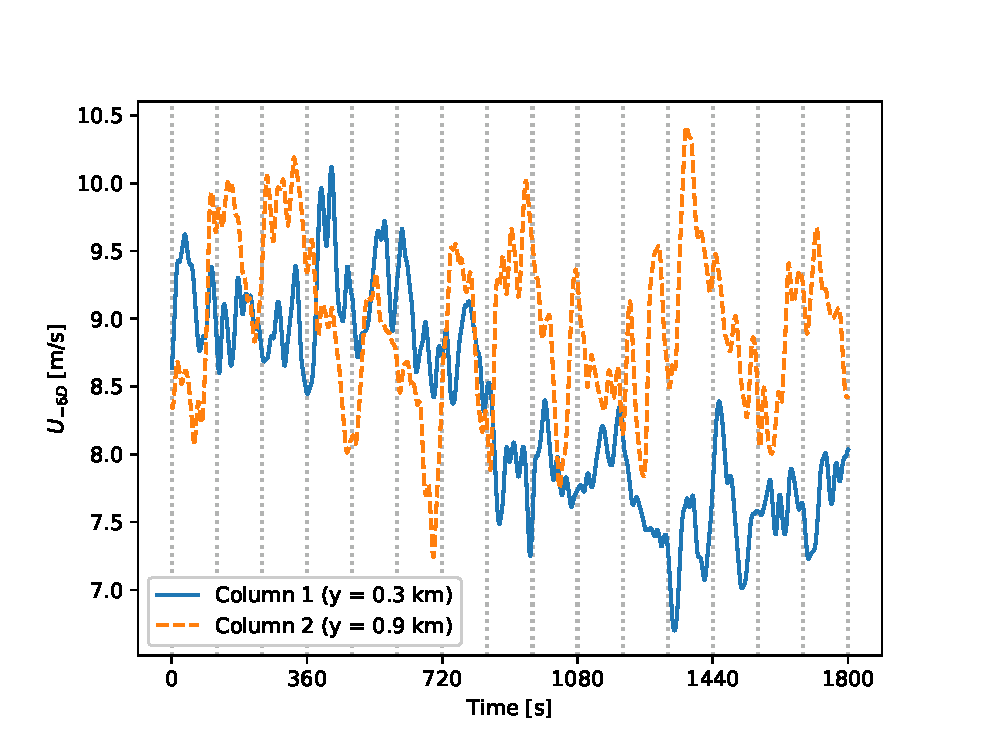
\includegraphics[width=\textwidth]{upstream_vel.eps}
	\caption{Disk-averaged axial velocity upstream of the first-row turbines for column 1 and column 2 in Figure 2 of the manuscript. Vertical dotted lines demarcate the optimization window boundaries (i.e. at integer multiples of $T_A$) \label{fig:upstream_vel}}
\end{figure}

\dotfill

\textbf{5. Reviewer: } \textit{On page 17, around line 5, a very nice example on how to implement the optimized
	sinusoidal CT is presented. The practical examples can be further improved by a
	short discussion on the expected response time of such increases in tip speed ratio
	on a machine with high inertia. That would put the estimated sine wave period into
	perspective as well.}

\textbf{Response: } We thank the reviewer for this suggestion. Dynamic reductions from the maximum $C_T' = 3.5$ could, for instance, be achieved by using the fast pitch actuators with which modern turbines are equipped. We have added this comment to the discussion as follows (p ??):  

``
The resulting maximum thrust coefficient of 3.5 can, e.g., be \textbf{attained by the NREL 5MW turbine with a slight modification in the rotor design}, i.e. a 50\% increase in blade chord length and an operational tip speed ratio 25\% higher than 
the original design value (see Goit and Meyers, 2015, Appendix A). \textbf{Furthermore, given such redesign, dynamic reductions from this value could be realized through blade pitch control, for which actuation in the order of $10^\circ/$s is possible (see, e.g., Jonkman et al. 2009).} 
''
 
Note that this control strategy is not unique and is solely given as an indication for the technical feasibility of tracking the proposed $C_T'$ waveform. In practice, we expect that this can also be achieved through a combination of generator torque and blade pitch control. This is subject of ongoing investigation.  

\dotfill

\textbf{6. Reviewer: } \textit{For Section 4.2.3, the header ``Full-scale wind farm test" is a bit misleading... Suggest
	to change to "Full-scale wind farm simulations (in LES)" instead.}

\textbf{Response: } Agreed, we have changed the section header to ``Full-scale wind-farm LES"

\dotfill

\textbf{7. Reviewer: } \textit{On Figure 19, why would the power decrease after Row 5 for the sinusoidal case?}

\textbf{Response: } This can be explained based on Figure 20: it can be seen from the cross-section views that by sinusoidally varying first-row thrust, the time-averaged axial velocity at the turbine disk for R2 is increased, but the flow above the turbine disk is actually slowed down, hence indicating that momentum is entrained from the internal boundary layer above the turbine canopy. In downstream rows, this high momentum zone expands and mixes with the background flow field. Starting from R5, this zone is almost completely dissipated, and the disk velocity is actually slighter lower than in the reference case. In short, the sinusoidal control actions of the first row actually entrain momentum from the surrounding flow that would otherwise be entrained by natural turbulent mixing further downstream in the wind farm. 

Moreover, it can be seen that the full optimal control (C3t5 in Figure 20) is able to contain the high momentum zone by continuously improving the mixing process with the background boundary layer. The mechanisms thereof however remain elusive to date, and are subject of further investigation. 

We have incorporated this discussion in the revised version of the manuscript as follows (p ?? l ??): 

``
... with higher rotor velocities in the downstream as well.  \textbf{Note also that, for the fifth row, the disk velocity is slightly lower for the sinusoidal control case than for the reference case, consistent with the decreased power extraction observed in Fig. 19. This can be explained by the fact that first-row control actions cause enhanced entrainment of momentum from the internal boundary layer above the turbine canopy that would otherwise be entrained by natural turbulent mixing in passive downstream rows. In consequence, lesser entrainment occurs for downstream rows, resulting in a slight decrease in disk velocities from the fifth row onwards.}
''

\dotfill

\textbf{8. Reviewer: } \textit{Page 22 around line 5, the (inevitable) discussions on loads are included. In addition
	to the loads on the controlled upstream turbine, Figure 20(b) indicates partial wakes
	on the further downstream rows of turbines. Therefore, the section should be improved
	by highlighting the probable increase in fatigue loading for not just turbine(s) R1 but for
	the downstream rows as well, possibly starting as early as R3.}

\textbf{Response: } We thank the reviewer for this comment. Agreed, the downstream turbines could also be subjected to increased fatigue loading, and we have included this in the revised manuscript as follows (p ??, l ??):

``
... to fatigue loading \textbf{of the first-row turbines. Furthermore, partial wake alleviation and unsteady passing of abovementioned vortex rings could also increase fatigue loading in downstream rows.} Hence, structural aspects ...
''

\dotfill

\textbf{9. Reviewer: } \textit{On the grammatical note, the manuscript is clear and easy to follow. The only comment
	might be on the use of Sect. or Section; Fig. or Figure references.}

\textbf{Response: } We have followed the official guidelines for referring to figures and sections as provided by the publisher, paraphrasing from the website:\

\emph{The abbreviation ``Sect.'' should be used when it appears in running text and should be followed by a number unless it comes at the beginning of a sentence.}\\({\small \verb|https://www.wind-energy-science.net/for_authors/manuscript_preparation.html|})

\end{document}
